\documentclass[11pt]{article}

\usepackage[utf8]{inputenc}
\usepackage[english]{babel}
\usepackage{hyperref}

\usepackage{amsmath}
\usepackage{physics}

\usepackage{graphicx}
\usepackage{caption}
\usepackage{subcaption}

\usepackage{listings}
\lstset{language=python}

\usepackage[style=nature]{biblatex}
\addbibresource{references.bib}

\title{Search and Task Allocation \\
    \small{Swarm Intelligence}}

\author{Sebastian G. Winther-Larsen}


\begin{document}
    
    \maketitle

    \section{Introduction}

    Search and Task Allocation (STA) problems are considered a general class of 
    problems in Multi-Agent Systems (MAS), and many real-world problems can 
    be formulated as an STA problem~\cite{ijspeert2001collaboration}.
    This is a study of reactive agents, where 
    we investigate how the introduction of communication impacts performance.

    \section{Formalism}

    We define a search $A$ as an area bound by two points. Over the search area, 
    $n_T$ tasks $T$ are spawned at random positions. The tasks have a task capacity
    $T_c$ indicating how many agents $R$ are required to solve a task. The task is 
    solved immeadeately if $T_c$ agents are within the task radius $T_r$.
    The agents $R$ move randomly around the search area at a speed $R_v$. There are 
    $n_R$ agents. When an agent is inside the task radius $T_r$ of a task, the agents 
    will wat for other agents to complete the task. The agents can also call for 
    aid in solving a task. The communication distance $R_d$ determines how 
    far an agent can send a call for aid from another agent.

    The position of the agents are updated in a discrete Langevinian manner,
    \begin{equation}
        \label{eq:langevinian}
        r_{R, t+1} = r_{R, t} + N\left(a_R +  b_{R, t}\right),
    \end{equation}
    where $r_{R, t}$ is the position of agent $R$ at time $t$, $a_r$ is a 
    drift term, $b_{R, t}$ is a stochastic velocity term and $N$ is a normalising
    operator, ensuring equal velocity of all agents. The drift term is assigned 
    at the start of each simulation and the stochastic velocity term is updated 
    for each time step. The trend is added in order to make sure that the agents
    will venture away from their origin point, as the expected value of 
    a sum of equally distributed stochastic variables with mean zero will be 
    zero. That is, even though there is a likelihood for agents to evetually 
    cover the entire area, one would expect them to meander about the point 
    they were initially placed.

    In addition to walking randomly across the area, the agents have the 
    possiblity of calling other agents in the vicinity, if they are within 
    a communication distance $R_d$.

    \section{Implementation} 

    We implement a tool for visualising the problem described above in 
    PyGame~\cite{pygame}.
    The full implementation is available at \url{github.com/gregwinther/mas},
    and consists of three classes. Two of these, \lstinline!Task! and \lstinline!Agent!,
    both inherit from PyGame's \lstinline!Sprite! class. The last class,
    \lstinline!Simulation!, takes care of the game mechanics such as updating
    states and drawing the area with tasks and agents. Initialising and running 
    a particular game (simulation) can be done with very few lines. For example;
    \begin{lstlisting}
        simulation = Simulation(1000)
        simulation.cycles = 1000
        simulation.communicate = True
        simulation.write = True
        simulation.n_T = 3
        simulation.Tr = 50
        simulation.n_R = 10
        simulation.Tc = 3
        simulation.start()
    \end{lstlisting}
    A screenshot of this example is shown in \autoref{fig:sample_screenshot}.

    \begin{figure}
        \centering
        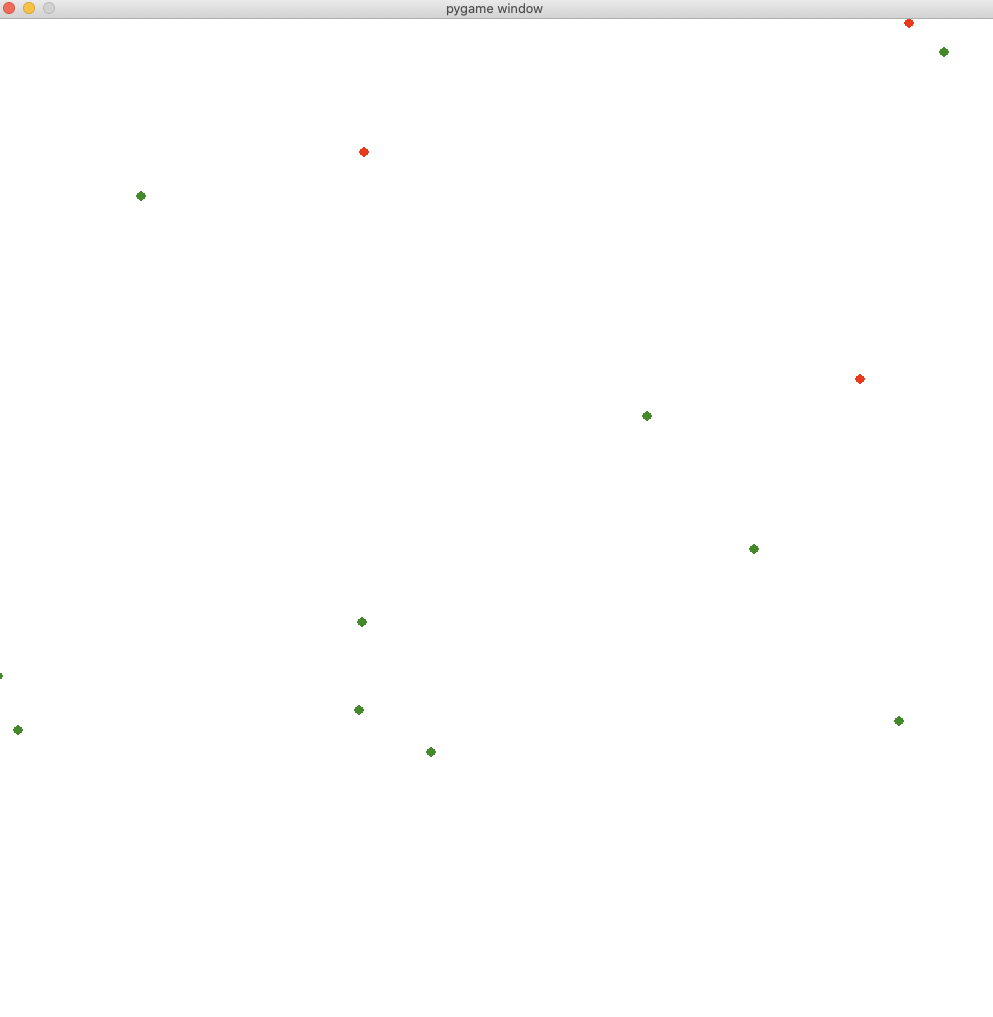
\includegraphics[width=0.8\textwidth]{figures/screenshot.png}
        \caption{
            Sample screenshot of a simulation with $n_T=3$ and $n_R=10$.
            The green dots are agents $R$, and the red 
            dots are tasks $T$. 
        }
        \label{fig:sample_screenshot}
    \end{figure}

    The most important methods of the \lstinline!Task! and \lstinline!Agent!
    classes is the \lstinline!update()! method, which is called for 
    each iteration of the game. For a Task, this method is 
    quite simple. It simple checks if there are enough agents within the 
    task radius $T_r$ to complete the task, if so the task sprite is killed.
    
    The \lstinline!update()! method for agents is more subtle. Firstly, it has to 
    update the positions of the agents according to \autoref{eq:langevinian}. 
    This is done by generating a random movement step, or finite difference velocity,
    which is added to the trend and then normalised to have lenght equal to $R_v$.

    Since it is possible for an agent to wander outside the area, we take care of 
    the boundaries in the following manner. When a moving agent hits one of the
    boundaries of the area, the trend unit vector which is perpendicular to 
    the boundary line is reversed. This has the effect of ``soft bounce'' 
    off the boundary.

    More than the mere movement of the agents, it is possible for them to be in
    different states. They may be \emph{searching}, \emph{tasked} or \emph{called}.
    The default state, \emph{searching}, is what we just described above. Whenever
    an agent is within the task radius $T_r$ of a task $T$ its state will change 
    to \emph{tasked}. If the task capacity $T_c$ required more agents than the
    one(s) present, the agent will stay put until enough agents arrive at the 
    task to help. With the mechanic enabled, an agent may also be \emph{called}
    if it is within the communication distance $R_d$ of another agent. The agent 
    will then move at speed towards the position of the signalling agent. When the 
    task is solved, the call will cease, in effect calling off any approaching agents.
    All of the transitions between agent states are handled within the main game loop 
    of the \lstinline!Simulation! class.

    \section{Results}

    All the simulations in this study is run five subsequent times in order to 
    get better averaged values, for a total of 1000 time steps. All simulations 
    also has the same task radius $T_r=50$.
    \autoref{fig:some_vs_many} shows the results of two arbitrary chosen sets
    of five simulations. The thin lines represent 
    the individual simulations, while the bold lines are the averages. For 
    both of these sets the number of tasks was $T_n=1$ with a task capacity $T_c=1$,
    while the number of agents $n_R$ are five and 20. The figure is meant to give 
    illustrate the necessity of repeated simulations in order to make 
    results separable.

    \begin{figure}
        \centering
        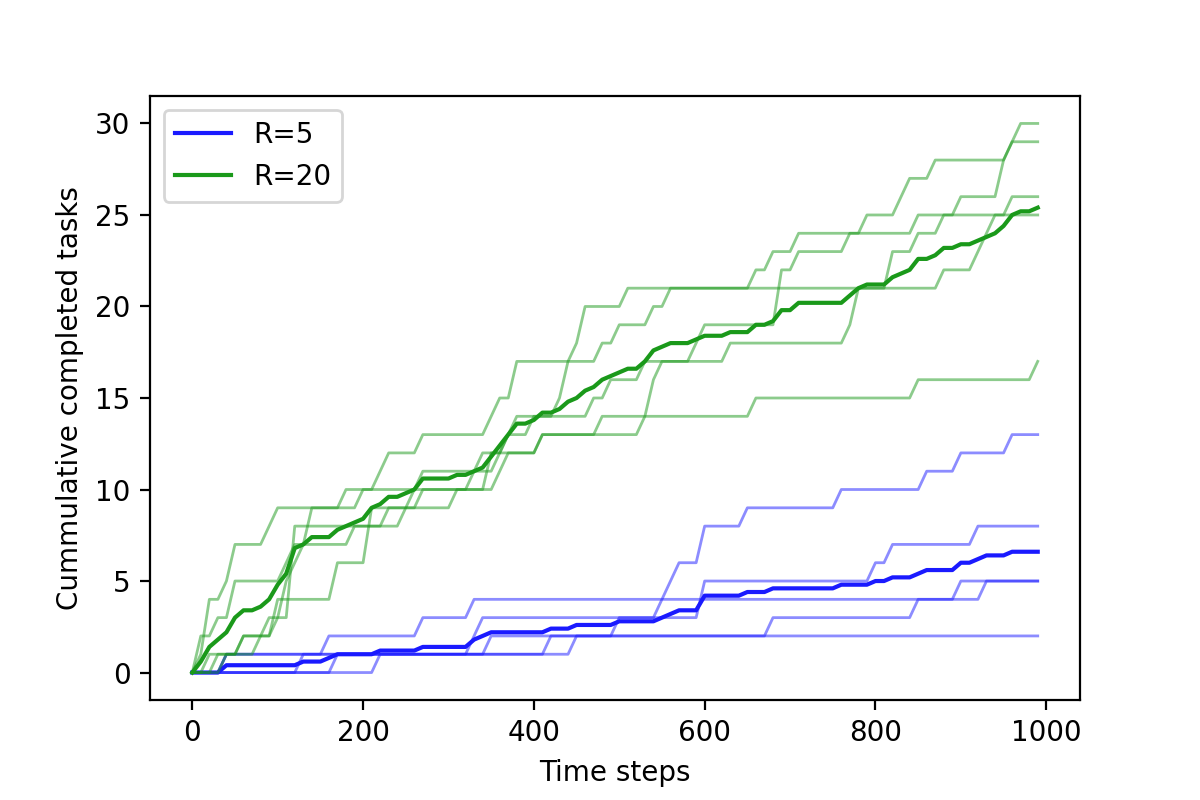
\includegraphics[width=0.7\textwidth]{figures/some_vs_many.png}
        \caption{
            Illustration of arbitrary simulations, with cumulative number 
            of solved tasks is plotted against the number of time steps.
            The number of tasks $T_n$ is 1 and the number of agents
            $R_n$ are 5 and 20. The task capacity $T_c$ was set to one.
            No communication was allowed in these simulations.
        }
        \label{fig:some_vs_many}
    \end{figure}

    To benchmark the system we run a number of simulations for various number 
    of tasks $T$ and number of agents $R$, with task capacity $T_c=1$. The 
    results of these simualtions are shown in \autoref{fig:tasks_vs_R}.
    The points indicate the average number of completed tasks at the end 
    of a simulation, with standard deviation given by the error bar.
    As expected, the number of completed tasks increase with the number 
    of agents $R$ and with the number of tasks $T$.

    \begin{figure}
        \centering
        \begin{subfigure}[b]{0.49\textwidth}
            \centering
            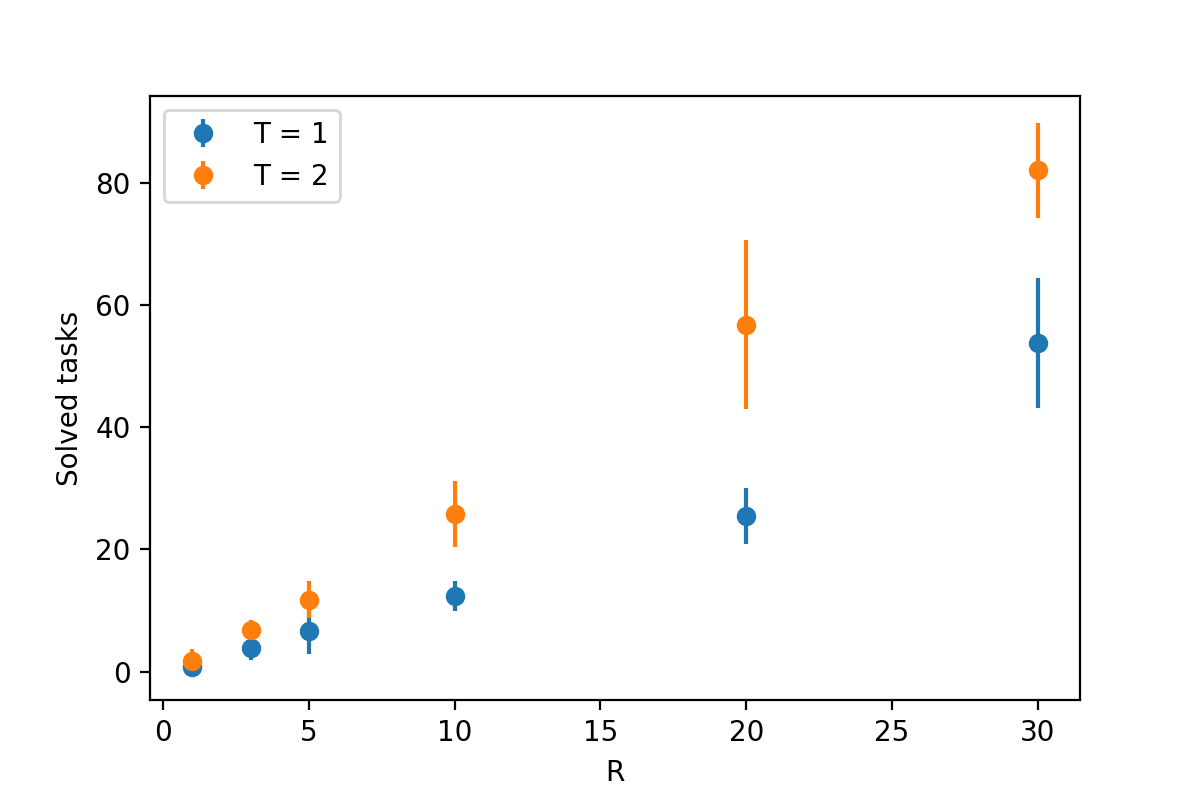
\includegraphics[width=\textwidth]{figures/low_T_tasks_vs_R.png}
        \end{subfigure}
        \hfill
        \begin{subfigure}[b]{0.49\textwidth}
            \centering
            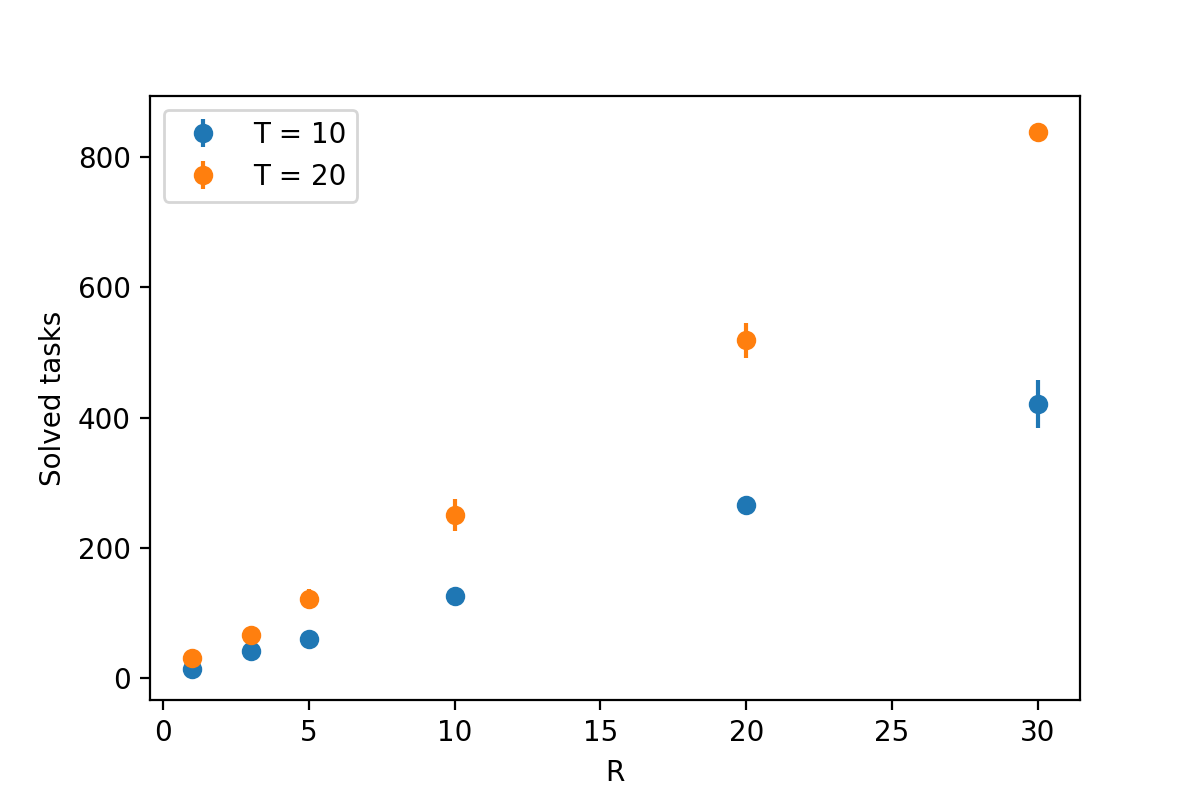
\includegraphics[width=\textwidth]{figures/high_T_tasks_vs_R.png}
        \end{subfigure}
        \caption{
            Completed tasks as a function of number of agents after 
            1000 time steps. The number of agents and tasks are varied, 
            while every other variable is held constant; $T_c=1$, $T_r=50$, 
            no communication.
        }
        \label{fig:tasks_vs_R}
    \end{figure}

    The results of introducing a higher task capacipy is depicted in
    \autoref{fig:Tc3_tasks_vs_R}. Here we set $T_c=3$, meaning that 
    three agents is needed to complete a task $T$. This figure is 
    comparable to the left-hand subfigure in \autoref{fig:tasks_vs_R}.
    We see a notably lower number of completed tasks when a task 
    capacity is introduced.

    \begin{figure}
        \centering
        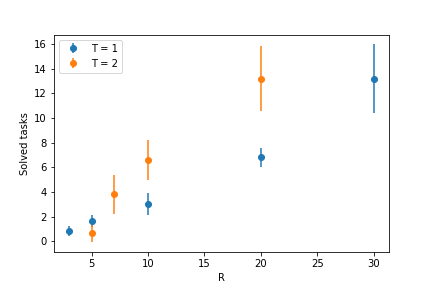
\includegraphics[width=0.7\textwidth]{figures/Tc3_tasks_vs_R.png}
        \caption{
            Completed tasks vs number of agents with $T_c=3$, for two different 
            task numbers $n_T \in \{1, 2\}$.
        }
        \label{fig:Tc3_tasks_vs_R}
    \end{figure}

    The results of introducing a call signal with reach $R_d=250$ can be 
    seen in \autoref{fig:call_vs_no_call}. The average performance is 
    markedly and significantly better when agents can call to others for help.

    \begin{figure}
        \centering
        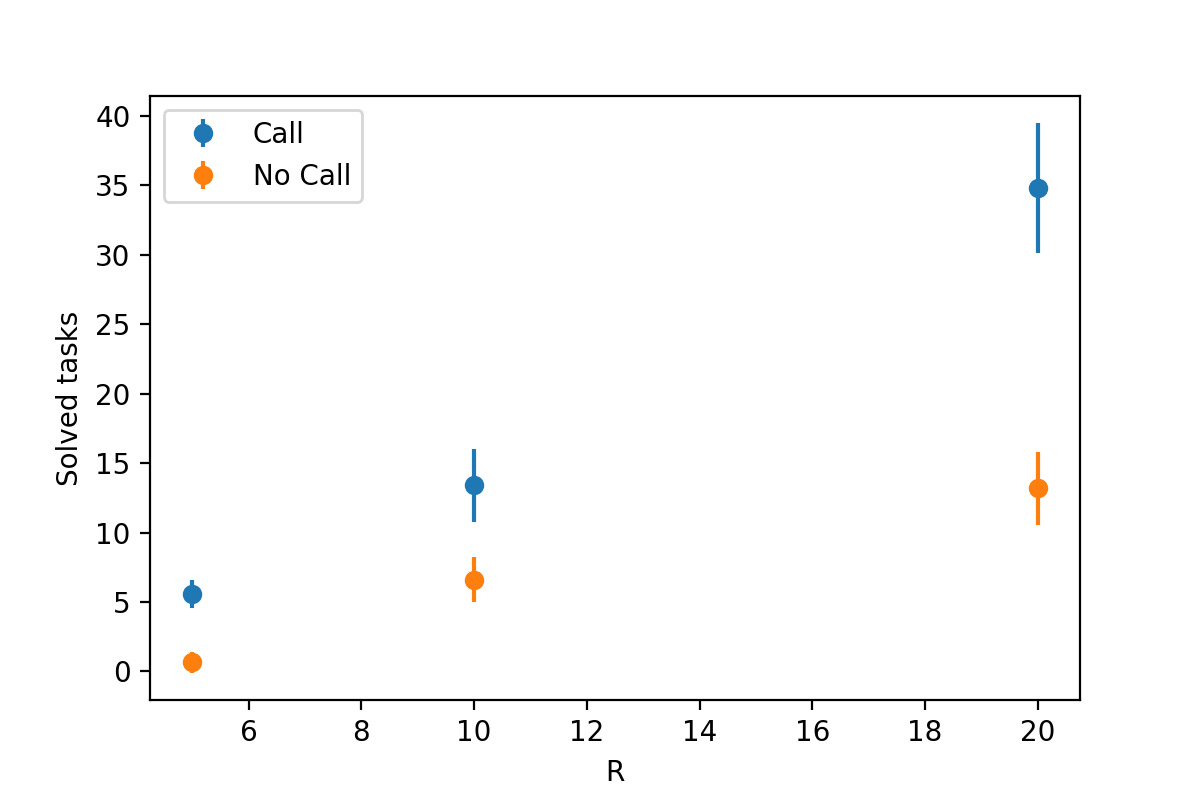
\includegraphics[width=0.7\textwidth]{figures/call_vs_no_call.png} 
        \caption{
            The effect of introducing a calling signal with $R_d=250$ when an 
            agent finds an agent finds a task. The number of tasks are $n_T=2$ 
            with capacity $T_c=3$.
        }
        \label{fig:call_vs_no_call}
    \end{figure}

    \autoref{fig:louder_call} shows the effect of increasing the communication 
    distance of the agents. The cumulative number of completed tasks is plotted 
    against time. In the simulations, only the communication distance is varied,
    $R \in \{250, 500, 1000\}$, all else equal ($T_c = 3$, $n_T=2$ and $n_R=5$).

    \begin{figure}
        \centering
        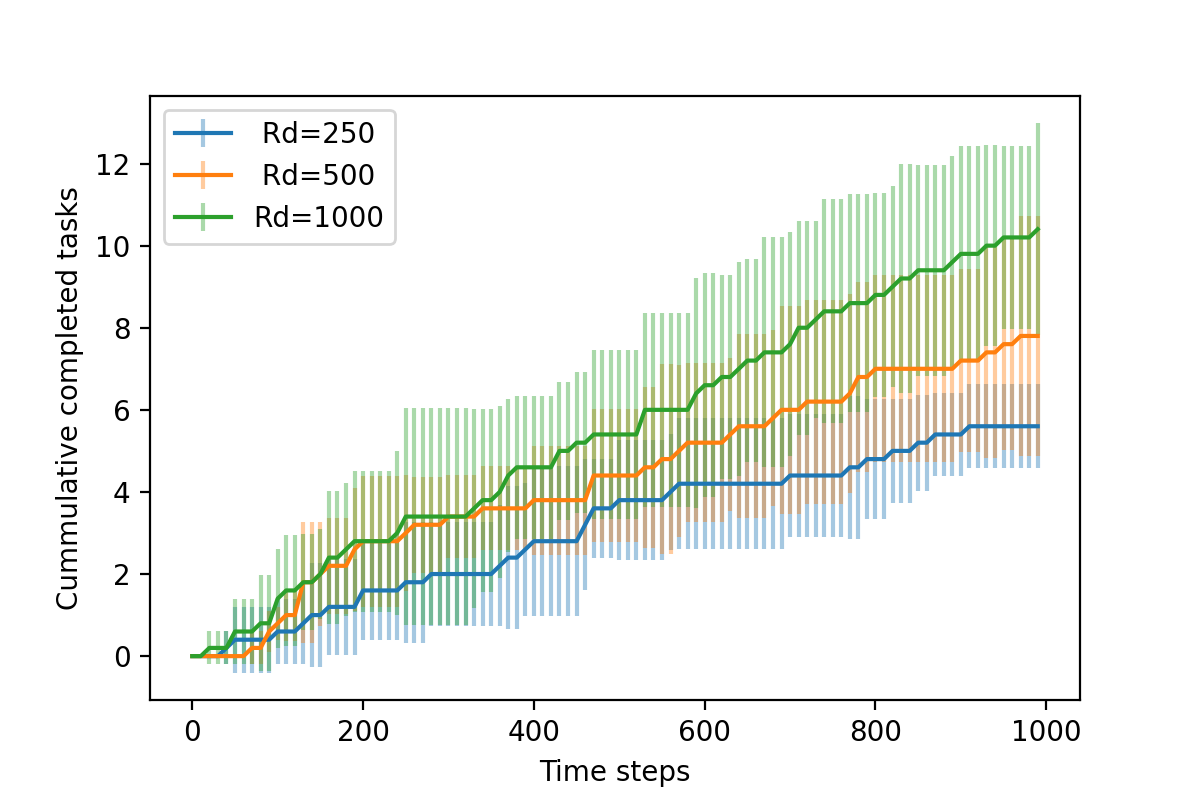
\includegraphics[width=0.7\textwidth]{figures/louder_call.png}
        \caption{
            Averages of three sets of five simulations for different 
            communication distances $R_d \in \{250, 500, 1000\}$,
            with $T_c = 3$, $n_T=2$ and $n_R=5$.
        }
        \label{fig:louder_call}
    \end{figure}

    \section{Discussion}

    In order to improve upon the stability of the initial searching of the agents,
    an improved pattern of movement could likely be devised. There are several
    improvements one could make when introducing communications, for instance to make
    the agents keep a distance to each other. There were several simualtions where many
    agents bunched up together.
    Another improvement with regards to communication 
    is to make sure that only the needed agents are called when a task is found. However,
    this would be a somewhat complicated alteration.
    A simpler improvement, would be to alter the drift 
    term of the agents over time in some clever way.
    As it is now, it stays the same, except for when 
    a boundary is reached. That said, it could be that a more deterministic movement 
    pattern is better at finding tasks than the random movement employed herein.
    
    Looking more closely at \autoref{fig:some_vs_many}, we see larger error bars 
    when there are fewer tasks.
    Because of the reduced probability of encountering a task with lower $n_R/n_T$
    ratio, the realtive uncertainty of these simulations are higher.
    A further study into the 
    necessity of either longer simulations or more simulations for a low 
    number of agents, is therefore warranted. 

    After the introduction of a task capacity, we encounter some ``sticky'' situations,
    especially as $n_T T_c \to n_R$, or more extremely when $n_T T_c \geq n_R$. In these situations,
    agents may find themselves waiting at a task until the end of the simulation, because 
    every other agent is also wating at a task. This leads to the interesting observation in 
    \autoref{fig:Tc3_tasks_vs_R} for $n_R=5$, where the performance is better for a lower number
    of tasks, which reduces the risk of agents getting ``stuck''. This could likely be improved 
    with a limited waiting time or the ability of an call-out from an agent to override a 
    task-solving agent.

    \printbibliography


\end{document}